%  article.tex (Version 1.00, released 1 October 2013)
%  LaTeX source file to demonstrate formatting for manuscripts 
%  to be submitted to SPIE journals
%  based on the class file spieman.cls, which requires 
%  the following standard packages:  times.sty, float.sty, 
%  ifthen.sty, cite.sty, color.sty, setspace.sty

%  The following commands have been added in the SPIE class 
%  file (spieman.cls) and may not be understood in other classes:
%  \affiliations{}, \sup{},\supit{}, \authorinfo{}, \keywords{},
%  \linkable and \video
%  The bibliography style file is called spiejour.bst 
%  This article.tex file needs the following image files:
%  mcr3b.eps
%  fig2.eps
%  satellite.eps

\documentclass[12pt]{spieman}  %>>> 12pt font mandatory; use this for US letter paper 
%%\documentclass[a4paper,12pt]{spieman}  %>>> use this instead for A4 paper
%%\documentclass[nocompress,12pt]{spieman}  %>>> to avoid compression of citations
%% \addtolength{\voffset}{9mm}   %>>> moves text field down
%  The following command loads a graphics package to include images 
%  in the document. It may be necessary to specify a DVI driver option,
%  for example, [dvips], but that may be inappropriate for some LaTeX installations. 
 
\usepackage[]{graphicx}
\usepackage{setspace}
\usepackage{tocloft}
\usepackage{units}
\usepackage{nicefrac}
\usepackage{color}
\usepackage{epstopdf}
\usepackage[globalcitecopy,labelstoglobalaux,sectionbib]{bibunits}
\usepackage[thinspace,thinqspace,squaren]{SIunits}
\usepackage{fancyhdr}
\usepackage{url}
\usepackage{wasysym}
%\usepackage{alltt}
%\renewcommand{\ttdefault}{txtt} 
\usepackage{array}
%\usepackage[version=3]{mhchem}
%\usepackage[T1]{fontenc}
%\usepackage{textcomp}
%\usepackage{verbatim} 
%\usepackage{mathpazo}
%\usepackage{amsmath} %>>> for AMS math formatting including bold Greek symbols
%\usepackage{mathtools}
\usepackage{amssymb}
\usepackage{accents}
\usepackage{url}
\usepackage{amscd}
\usepackage{epsfig}
\usepackage{cite}
\usepackage{subfig}
\usepackage[globalcitecopy,labelstoglobalaux,sectionbib]{bibunits}
%\usepackage[sectionbib]{bibunits}
\usepackage{appendix}
\usepackage{slashbox}
%\usepackage{multirow}
%\usepackage{caption}

\title{Working title: the most amaz-zing SPIM and how we built it. Authors currently alphabetical.} 

\author{Irene Costantini,\supscr{a} Giulio Iannello,\supscr{d} M. Caroline M\"{u}llenbroich,\supscr{a} Leonardo Onofri,\supscr{d} Francesco S. Pavone,\supscr{a,b,c} Leonardo Sacconi,\supscr{b,a} Ludovico Silvestri, \supscr{a} Marcel Van t'Hoff\supscr{x}}

\affiliation{\supscrsm{a}European Laboratory for Non-linear Spectroscopy, University of Florence, Via Nello Carrara,1, Sesto Fiorentino (Firenze), Italy, 50019\\
\supscrsm{b}National Institute of Optics, National Research Council, Italy\\
\supscrsm{c}Department of Physics and Astronomy, University of Florence, Via Giovanni Sansone, 1, Sesto Fiorentino (Firenze), Italy, 50019\\
\supscrsm{d}Integrated Research Centre, University Campus Bio-Medico of Rome, Italy\\
\supscrsm{x}Distrio, Murmex}

%%%%%%%%%%%%%%%%%%%%%%%%%%%%%%%%%%%%%%%%%%%%%%%%%%%%%%%%%%%%% 
\renewcommand{\cftdotsep}{\cftnodots}
\cftpagenumbersoff{figure}
\cftpagenumbersoff{table} 
\begin{document} 
\maketitle 

%%%%%%%%%%%%%%%%%%%%%%%%%%%%%%%%%%%%%%%%%%%%%%%%%%%%%%%%%%%%% 
\begin{abstract}
200 words limit. no numerical references presenting concisely the objectives, methodology used, results obtained, and their significance.
\end{abstract}

%>>>> Include a list of up to six keywords after the abstract
\keywords{Light sheet microscopy, Big data, Optical clearing, Data management, whole brain imaging, rolling shutter, 7,8.}

%>>>> Include contact information for corresponding author
{\noindent \footnotesize{\bf Address all correspondence to}: First author, University Name, Faculty Group, Department, Street Address, City, Country, Postal Code; Tel: +1 555-555-5555; Fax: +1 555-555-5556; E-mail:  \linkable{myemail@university.edu} }
%%%%%%%%%%%%%%%%%%%%%%%%%%%%%%%%%%%%%%%%%%%%%%%%%%%%%%%%%%%%%

\begin{spacing}{2}   % use double spacing for rest of manuscript

%%%%%%%%%%%%%%%%%%%%%%%%%%%%%%%%%%%%%%%%%%%%%%%%%%%%%%%%%%%%%
\section{Introduction}
\label{sect:intro}  % \label{} allows reference to this section
Here will be an introduction to whole brain imaging the challenges it is facing and how light sheet microscopy is addressing those challenges. Points to raise: briefly optical clearing, big data generation and management, image quality degradation necessitating rolling shutter, refocusing?, The next parts will be in clear sections so that we can divide them better between us if necessary. Can be merged later on if we wish so.

Basic principles of light sheet microscopy: light efficiency/reduced phototoxicity, speed, true optical sectioning, resolution etc.

\section{Optical clearing}
CLARITY and TDE stuff, get contribution/input from Irene.

\section{Optomechanics}
	\subsection{Optical path}
Here we describe our optical setup, the components we use etc. 
		\subsubsection{illumination}
		lasers, AOTF, Pockels, Bessel, double sided, digitally scanned, objectives
		\subsubsection{detection}
		objective, camera, rolling shutter. Use references\cite{Silvestri2012} to old SPIM.
		\subsubsection{Sample mounting and rotation}
		the sample chamber is probably of particular interest, how was it designed and made, how do we protect the objectives, stop it from leaking, soft connections and hard connections. how do we rotate and move the sample within the chamber. in the end, this is where the magic happens....

	\subsection{Alignment}
and maybe also some details on how we aligned everything. we have our sample mirror with the hole in it, the shear plate, periscopes etc...

	
\section{Software Management}
Here we describe all things software control and communication, components and their interaction. how is the rolling shutter timed with galvos, triggers and clocks etc. Get in touch early with Marcel to ask him and write/contribute to this paragraph.

\section{Data Management}
	\subsection{Pipeline}
	Here we describe our data pipeline: data production rate as function of frame rate and image size, stack size, tomo size, SSD space, transfer to NAS digital downsampling, and tiff compression, Leo's python script, NAS to CINECA, 10 gigabit connection etc.

	\subsection{stitching and visualisation}
	Terastitcher and Teraviewer

	\subsection{example for postprocessing: Automated cell counting}
	See Reference\cite{Frasconi2014} for details.


\section{Data}
some pretty images to prove that it all worked.

\section{Conclusion}
summary

\section{Outlook}
where are we going next with this? 

%%-------------
   %\begin{figure}
   %\begin{center}
   %\begin{tabular}{c}
   %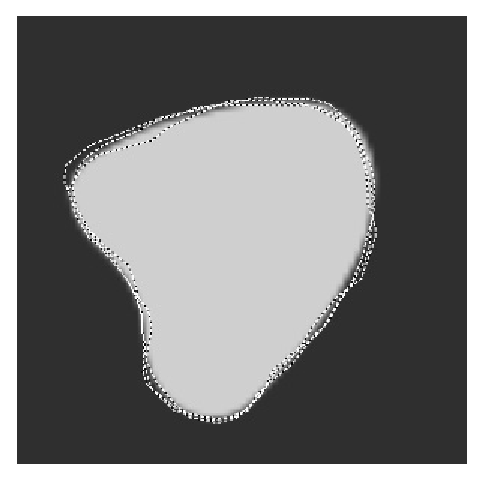
\includegraphics[height=5.5cm]{mcr3b.eps}
   %\end{tabular}
   %\end{center}
   %\caption 
   %{ \label{fig:example} %>> use \label inside caption to get Fig. number with \ref{}
%Example of a figure caption. } 
   %\end{figure} 
%
%%------------- 
   %\begin{figure}
   %\begin{center}
   %\begin{tabular}{c}
   %
\includegraphics[height=5.5cm]{fig2.eps}  % fig2 includes two images 
     %\\
     %(a) \hspace{5.1cm} (b)
   %\end{tabular}
   %\end{center}
   %\caption 
   %{ \label{fig:example2} %>> use \label inside caption to get Fig. number with \ref{}
%Example of a figure containing multiple images: (a) sun and (b) blob. Figures containing multiple images must be submitted to SPIE as a single image file.} 
   %\end{figure} 

%%%%%%%%%%%%%%%%%%%%%%%%%%%%%%%%%%%%%%%%%%%%%%%%%%%%%%%%%%%%%
\acknowledgments 
Human Brain Project tutta la vita. 

%%%%%%%%%%%%%%%%%%%%%%%%%%%%%%%%%%%%%%%%%%%%%%%%%%%%%%%%%%%%%
%%%%% References %%%%%

%\bibliography{report2}   %>>>> bibliography data in report.bib
\bibliographystyle{spiejour}   %>>>> makes bibtex use spiejour.bst
\begin{thebibliography}{0}

\bibitem{Silvestri2012} Silvestri, L., Bria, A., Sacconi, L., Iannello, G. \& Pavone, F. S. 	\emph{Opt Express} \textbf{20}, 20582-20598 (2012).

\bibitem{Frasconi2014} Frasconi, P., Silvestri, L., Soda, P., Cortini, R., L., Pavone, F. S., \& Iannello, G. 	\emph{Bioinformatics} \textbf{30}, i587-i593 (2014).


\end{thebibliography}


\listoffigures
\listoftables

\end{spacing}
\end{document} 
